% Cupid Overview and Tutorial
% Rocky Dunlap

\documentclass[oneside,11pt]{memoir}

\settrimmedsize{11in}{210mm}{*}
\setlength{\trimtop}{0pt}
\setlength{\trimedge}{\stockwidth}
\addtolength{\trimedge}{-\paperwidth}
\settypeblocksize{7.75in}{33pc}{*}
\setulmargins{4cm}{*}{*}
\setlrmargins{1.25in}{*}{*}
\setmarginnotes{17pt}{51pt}{\onelineskip}
\setheadfoot{\onelineskip}{2\onelineskip}
\setheaderspaces{*}{2\onelineskip}{*}
\checkandfixthelayout

\usepackage{titlepic}
\usepackage{hyperref}
\usepackage{graphicx}
%\usepackage{color}
%\usepackage{xcolor}
\usepackage{listings}
%\usepackage{caption}

% source code listing captions
%\DeclareCaptionFont{white}{\color{white}}
%\DeclareCaptionFormat{listing}{\colorbox{gray}{\parbox{\textwidth}{#1#2#3}}}
%\captionsetup[lstlisting]{format=listing,labelfont=white,textfont=white}

% source code listings
\lstset{
	language=Fortran,
	basicstyle=\small\sffamily,
	%basicstyle=\footnotesize\ttfamily,
	numbers=left,
	numberstyle=\tiny,
	frame=tb,
	columns=fullflexible,
	showstringspaces=false
}

% macros for formatting
\newcommand{\mapping}[1]{\texttt{\textit{#1}}}

%%%%%%%%%%%%%%%%%%
% document start %
%%%%%%%%%%%%%%%%%%

\begin{document}

\title{The Cupid Integrated Development Environment for Earth System Models}
\author{Rocky Dunlap\thanks{This work supported by the NASA CMAC program.}\\
	College of Computing\\
	Georgia Tech\\
	\texttt{rocky@cc.gatech.edu}}
\date{\today}
\titlepic{
\includegraphics{figs/logo_cupid.png}}


\maketitle



\clearpage
\tableofcontents

\chapter{Overview of Features}

Cupid is a set of development tools to facilitate the adoption of the geoscience modeling frameworks into new and existing model codebases.  The target framework is the \href{http://www.earthsystemmodeling.org/}{Earth System Modeling Framework} (ESMF) and its interoperability layer called the \href{https://earthsystemcog.org/projects/nuopc/}{National Unified Operation Prediction Capability} (NUOPC), which is currently being implemented in most major climate and weather models in the US. Cupid tools are intended for model developers who have prior experience with model development workflows, but are new to developing with ESMF and NUOPC.  It is also aimed at developers interested in exploring the benefits of using the Eclipse Integrated Development Environment (IDE) for improving development productivity.

Use of modeling frameworks is quickly becoming the norm for both operational and research climate and weather models. Modeling frameworks provide a number of benefits including mechanisms for componentizing complex codebases, functions and data structures for coupling independent models into a single simulation, increased developer productivity through code reuse, improved quality and robustness of features compared with ``home grown'' solutions, and fast execution via parallel data transfer and interpolation operators. 

In a framework-based application, such as a coupled model that uses ESMF, some application behaviors are provided by the framework and some are provided by the application developer. For example, ESMF provides functions for transferring and interpolating field data from one model's native grid to another model's native grid. However, ESMF does not prescribe what it means for the model to take a step forward in time since that behavior is application specific. The framework provides a set of abstractions, \emph{framework-provided concepts}, that the developer is required to instantiate and configure in their code. Creating a framework-based application is called \emph{framework completion} because the developer fills in application behaviors not provided by the framework, or specializes  behaviors provided by the framework. 

The Cupid tools adds framework-specific intelligence to the \href{https://www.eclipse.org/}{Eclipse Integrated Development Environment} in order to facilitate adoption of ESMF and NUOPC. The features include:
\begin{itemize}

\item A tool for \textbf{reverse engineering} an existing codebase to determine what ESMF and NUOPC framework concepts are present in the code. The reverse engineering function does not require execution of the user's code---instead, it operates during the phase of development when code is written, such as when framework code is first introduced into an existing model. The reverse engineered model is presented to the user alongside the source code in the form of a tree where nodes correspond to framework concepts. Clicking on a node takes the user directly to the relevant code fragments. The reverse engineering tool also checks for code-level compliance to \href{https://earthsystemcog.org/projects/nuopc/esmf2nuopc}{NUOPC technical rules} and offers suggestions for addressing compliance issues.

\item A tool for \textbf{automatic source code generation} of NUOPC-compliant code fragments directly in new or existing source files.  The generated code helps the developer see what framework concepts should be instantiated in their code, such as framework functions the developer should call, callback functions that the developer must implement, and what API methods are relevant in particular contexts.

\item A \textbf{cloud configuration} feature that allows the user to select a training scenario and, within a few minutes, configure, compile, execute, and view the output of both skeleton models and realistic models executing on virtual machine instances on the \href{http://aws.amazon.com/ec2/}{Amazon EC2} platform.

\end{itemize}

\chapter{ESMF and NUOPC}

This section describes the Earth System Modeling Framework (ESMF) and the National Unified Operational Prediction Capability (NUOCP) and provides references for those interested in finding out more. Readers already familiar with ESMF and NUOPC may choose to skip this section.

\section{The Earth System Modeling Framework}
ESMF is a high-performance software framework designed for numerical geoscience models. Some of the framework-provided concepts include model components (\texttt{ESMF\_GridComp}) and coupler components (\texttt{ESMF\_CplComp}; mediators between model components), and data types for model state (\texttt{ESMF\_State}), distributed arrays (\texttt{ESMF\_Array}), physical fields (\texttt{ESMF\_Field)}, and numerical grids (\texttt{ESMF\_Grid}; discretization schemes). An ESMF-based application is typically designed as a hierarchy of model components where components communicate by exchanging \texttt{ESMF\_State} objects via framework-provided interfaces. \texttt{ESMF\_GridComp}s and \texttt{ESMF\_CplComp}s have user-customizable \texttt{initialize()}, \texttt{run()}, and \texttt{finalize()} methods.  For more information about ESMF, see the \href{http://www.earthsystemmodeling.org/esmf_releases/public/last/ESMF_usrdoc/}{ESMF User's Guide} and the \href{http://www.earthsystemmodeling.org/esmf_releases/public/last/ESMF_refdoc/}{ESMF Reference Manual}.

\section{The National Unified Operational Prediction Capability}
To promote interoperability of model components, NUOPC is a set of generic components, metadata conventions, and behavioral protocols encoded in a software layer on top of ESMF. Together, these elements form the basis of a \emph{common model architecture}---a standard way of building models in order to make it easier to assemble coupled models using components from different sources. NUOPC is currently being implemented in research and operational models such as the HYCOM ocean model~\cite{hycom}, GFDL's MOM5 ocean model~\cite{mom5}, and NASA's ModelE climate model~\cite{modele}.  Additional information about NUOPC can be found on the \href{https://earthsystemcog.org/projects/nuopc/}{NUOPC home page}.

%Cupid is a tool that aids model developers in creating, executing, and analyzing Earth System Modeling Framework (ESMF) codebases that adhere to the conventions defined by the National Unified Operational Prediction Capability (NUOPC), a software layer designed to facilitate interoperability of modeling components used in operational weather prediction systems.  Cupid is implemented as a plugin for the Eclipse Integrated Development Environment\footnote{http://www.eclipse.org} and leverages existing plugins, especially the Photran language editor\footnote{http://www.eclipse.org/photran/}.

NUOPC applications are built by combining four basic building blocks called \emph{generic components}. The four types of generic component are \texttt{Driver}, \texttt{Model}, \texttt{Mediator}, and \texttt{Connector}. Many component behaviors have been predefined by NUOPC. However, in some cases, the developer needs to provide implementations of behaviors not defined by NUOPC. Additionally, if the generic behavior does not meet the requirements of the coupled model, the developer may need to override existing behaviors.  In both cases, the developer's implementation is typically provided in subroutines which are registered with and called by the framework. The process of providing new behaviors or overriding existing ones is called \emph{specialization}. As defined here, \emph{specialization} is conceptually similar to how a class overrides a parent class method to provide a different implementation in an object-oriented programming language. However, because the public ESMF and NUOPC APIs are not implemented in an object-oriented language, a custom specialization mechanism has been defined. Understanding the specialization process is essential for adopting NUOPC into a model's codebase.

The \texttt{Driver} generic component implements a harness of ESMF components and \texttt{ESMF\_State} objects and it is specialized by plugging in \texttt{Model}, \texttt{Mediator}, \texttt{Connector}, and other \texttt{Driver} components. The \texttt{Driver} initializes its child components according to an \emph{Initialize Phase Definition} and drives their \texttt{run()} methods according to a \emph{Run Sequence}. \texttt{Model} wraps a user's code so it can be plugged into a \texttt{Driver}. \texttt{Model}s represent major geophysical domains such as atmosphere, ocean, and ice. \texttt{Connector}s and \texttt{Mediator}s manage communication between \texttt{Model}s. \texttt{Connector}s implement standard interactions such as parallel redistribution or regridding (interpolation) of fields and \texttt{Mediator}s implement complex \texttt{Model} interactions requiring customized code. Figure~\ref{fig:nuopcarchs} illustrates several possible architectural configurations of NUOPC components.

\begin{figure}
	\centering
	 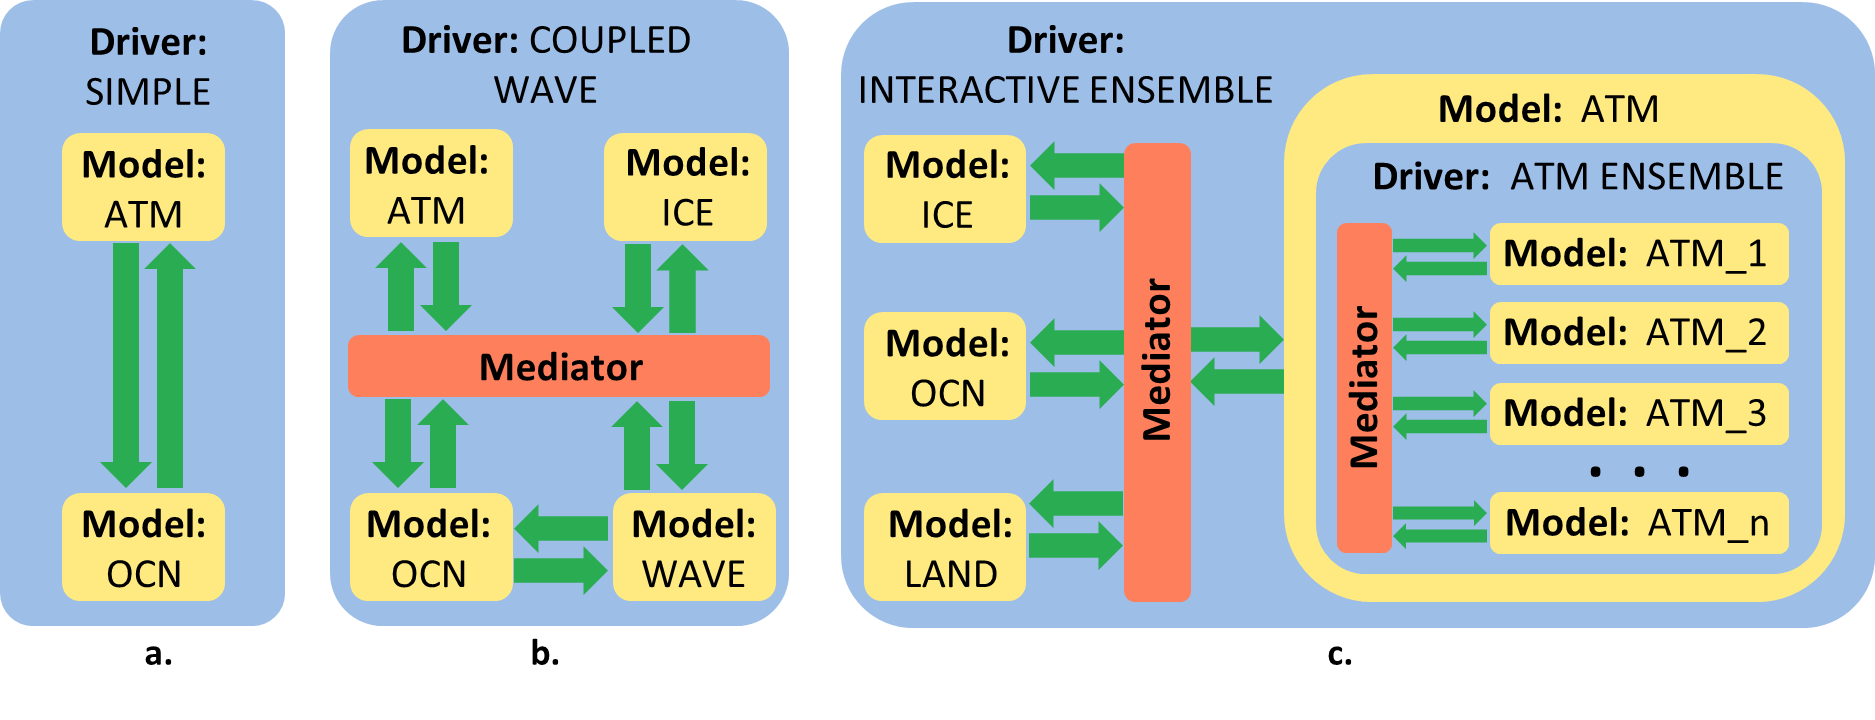
\includegraphics[width=\textwidth]{figs/nuopcarchs.png}
	\caption{\textbf{a.} A \texttt{Driver} (blue box) with two child \texttt{Model}s (yellow boxes) and simple \texttt{Connector}s (green arrows).  \textbf{b.} A configuration in which a \texttt{Mediator} (orange box) couples atmosphere, ocean, ice, and wave \texttt{Model}s.  \textbf{c.} A complex configuration showing nested \texttt{Driver}s.}
	\label{fig:nuopcarchs}
\end{figure}

To take full advantage of NUOPC, developers must ensure that model components comply with NUOPC architectural constraints and technical rules. The full definition of NUOPC compliance is available on the \href{http://earthsystemcog.org/projects/nuopc/esmf2nuopc}{NUOPC compliance web page}. 

%Cupid supports the goals of NUOPC by providing a tool capable of generating fragments of framework completion code (while not hindering developers from writing customized code) and validating existing NUOPC codebases.

\chapter{Reverse Engineering and Compliance Verification of NUOPC Applications}

Most climate and weather model codebases are staggeringly large and obtaining an overview of the model, its subcomponents, and their interconnections is a cumbersome, time-consuming task. Often, this can only be accomplished by manually reading through the top-level source files to establish a mental picture of the overall structure of the model and its data flows. 

Instead of viewing a model as an opaque, complex set of source files, Cupid's reverse engineering feature parses a model's source code and produces an abstract representation of the framework concepts that are present in the code. The reverse engineering feature is a kind of \href{http://en.wikipedia.org/wiki/Static_program_analysis}{static analysis} because the source code is analyzed before it is compiled and does not require execution of the model.  This representation is shown to the user alongside the source code in an outline form called the NUOPC tree viewer. This provides an alternative, more abstract perspective for viewing a model’s source code. Some of the main concepts provided by NUOPC are Drivers, Models, Mediators, and Connectors. If a codebase contains any of these generic components, the reverse engineering function will automatically find them and present them in outline form. This provides an architectural overview of an entire coupled system without requiring the developer to read through thousands of lines of source code.

NUOPC ensures interoperability of modeling components by specifying a set of technical rules that model implementers should follow.  In addition to presenting a high level view of framework concepts in source code, Cupid’s compliance checking feature provides feedback to the user when potential compliance issues are discovered in a reverse engineered model. For example, when developing a NUOPC Model component, certain subroutines must be implemented and registered with the framework. If a required subroutine or its registration is missing, Cupid can identify the problem and annotate the outline view with icons indicating that some required code is missing. Moreover, this feedback is provided immediately to the user during model development thereby reducing the number of runtime failures and improving efficiency of the development process.


\chapter{Generating NUOPC-compliant Code}

Even if a software framework is well designed, writing framework completion code is notoriously difficult, even for seasoned developers. Often, completing a single logical task such as adding a new run initialization phase or run phase to the model requires making several code additions at multiple places spread throughout the application source code. If one or more of the required additions are inadvertently left out, the application may not behave as expected.  
In the software engineering research community, many ideas have been proposed for how to help developers write framework-based applications correctly and efficiently. For ESMF and NUOPC, guidance is provided in the form of comprehensive API documentation (\href{http://www.earthsystemmodeling.org/esmf_releases/public/last/ESMF_refdoc/}{ESMF}, \href{https://earthsystemcog.org/projects/nuopc/refmans}{NUOPC}), system tests (included with source distribution), and \href{https://earthsystemcog.org/projects/nuopc/proto_codes}{small archetypical codebases} that show how to structure NUOPC applications based on the components in the modeled system (e.g., standalone atmosphere, coupled atmosphere-ocean, three-component system, etc.). 

Cupid's code generation feature complements these static resources by generating on-the-fly NUOPC-compliant source code fragments directly in existing source files. The user initiates a code fragment generation by adding elements to a reverse engineered model in the NUOPC tree viewer. The source code is then synchronized with the tree viewer, generating the required code fragments. The generated code fragments can then be customized by the developer for their particular case. The following use case illustrates use of forward engineering feature:

\begin{quote}
A developer has finished writing the initialization phases for a NUOPC Model component called ATM and now needs to add the capability to advance the model one time step. The developer right clicks on the ATM element in the NUOPC tree viewer and selects ``Add Model Advance.''  Two things happen immediately: the tree viewer is updated with a new sub-element underneath ATM called ``Model Advance'' which in turn contains sub-elements ``Registered in Set Services'' and ``Implementation.'' Then, source code fragments are generated inside the Fortran file for ATM including a call inside the ATM SetServices to register the Model Advance subroutine and a stub for the new Model Advance subroutine.
\end{quote}

The use case shows some advantages of this approach compared to an approach in which code is copied-and-pasted from archetypical example code. First, the new Model Advance element added to the tree viewer included multiple sub-elements indicating that source code changes are required in at least two places: a new subroutine and a call to register this subroutine with the framework.  This provides guidance to the developer to ensure that all framework requirements are met. The approach, therefore, is less error-prone than brute force copy and paste. Also, the generated code fragments are customized based on the state of the existing source code. For example, the developer may be using specialized variable names. Since these variables have already been discovered during the reverse engineering phase, the generated code can reference these variables instead of requiring the developer to modify variables in copy-pasted code.


\chapter{Cloud-based configuration}

Cupid simplifies the process of configuring a computational environment capable of compiling and executing high-performance geoscience models. IDEs package a lot of development tools into a single application to help manage and simplify the software development workflow. Although IDEs aim to increase developer productivity, they can still introduce a steep learning curve. Some challenges with using IDEs for geoscience model development include:

\begin{itemize}
\item Understanding the basic steps involved in moving from source code to a running model
\item Making sense of the many development tools and features available in the IDE
\item Setting up a high-performance computational environment capable of configuring, compiling and executing model code
\item Configuring the IDE to connect to remote computational environments
\end{itemize}

Cupid's cloud integration feature allows a developer to select a training scenario and, within a few minutes, configure, compile, execute, and view the output of both skeleton models and realistic models. This feature relies on a set of pre-configured machine images that can be instantiated on Amazon EC2 cloud infrastructure. The machine images contain all of the necessary software dependencies for the selected scenario. Furthermore, Cupid automatically configures the IDE to connect to and synchronize source code with cloud-based virtual machines.


\chapter{The Behind-the-Scenes Meta-tool}
%In general, a software framework provides a set of abstractions, \emph{framework-provided concepts}, which the developer is required to instantiate and configure in code. Creating a framework-based application is called \emph{framework completion} because the developer is filling in application behaviors not provided by the framework, or specializing existing behaviors. 

This section describes theoretical and implementation aspects of the meta-tool used to define the mappings from framework-provided concepts to source code. This chapter may be of interest to software engineering researchers or those interested in using Cupid for defining their own framework-specific development tools. Reading this chapter is optional for users who wish to use the tool to develop NUOPC-based applications.

To support model developers in writing NUOPC-complaint code, the Cupid tool leverages existing work aimed at facilitating development of framework-based applications called Framework-Specific Modeling Languages (FSMLs). A FSML is a domain-specific language designed for a specific framework \cite{antkiewicz06}. FSMLs are aimed at addressing some of the challenges involved in developing framework-based applications, especially knowing how to complete a framework correctly and how to ensure respect of its rules of engagement\cite{antkiewicz06}. The language elements in the FSML's abstract syntax represent framework-provided concepts that the developer instantiates in code. FSMLs can be represented as a \emph{feature model}~\cite{czarnecki}, where features correspond to framework-provided concepts and each feature model configuration represents a valid framework completion.

Bidirectional mappings from framework-provided concepts to application source code are used to support forward and reverse engineering functions. In the forward direction, framework completion code is generated from an FSML instance---i.e., a Framework-Specific Model (FSM). In the reverse direction, an existing codebase is analyzed in order to recognize code patterns that correspond to framework concepts, producing a FSM. Taken together, the forward and reverse mappings enable round-trip engineering: the developer can seamlessly move between two perspectives, a zoomed in code-level perspective for customizing source code, and a higher level perspective showing the framework concepts present in the application and their inter-relationships. 


%\begin{lstlisting}[label=NUOPCCode, caption=A typical SetServices subroutine for a specialized \texttt{NUOPC\_Model}]
%subroutine SetServices(gcomp, rc)
    %type(ESMF_GridComp)  :: gcomp
    %integer, intent(out) :: rc
    %
    %rc = ESMF_SUCCESS
    %
    %! the NUOPC model component will register the generic methods
    %call model_routine_SS(gcomp, rc=rc)
    %if (ESMF_LogFoundError(rcToCheck=rc, msg=ESMF_LOGERR_PASSTHRU, &
      %line=__LINE__, &
      %file=__FILE__)) &
      %return  ! bail out
%
    %! set entry point for methods that require specific implementation
    %call ESMF_GridCompSetEntryPoint(gcomp, ESMF_METHOD_INITIALIZE, &
      %userRoutine=InitializeP1, phase=1, rc=rc)
    %if (ESMF_LogFoundError(rcToCheck=rc, msg=ESMF_LOGERR_PASSTHRU, &
      %line=__LINE__, &
      %file=__FILE__)) &
      %return  ! bail out
    %call ESMF_GridCompSetEntryPoint(gcomp, ESMF_METHOD_INITIALIZE, &
     %userRoutine=InitializeP2, phase=2, rc=rc)
    %if (ESMF_LogFoundError(rcToCheck=rc, msg=ESMF_LOGERR_PASSTHRU, &
      %line=__LINE__, &
      %file=__FILE__)) &
      %return  ! bail out
    %
    %! attach specializing method(s)
    %call ESMF_MethodAdd(gcomp, label=model_label_Advance, &
      %userRoutine=ModelAdvance, rc=rc)
    %if (ESMF_LogFoundError(rcToCheck=rc, msg=ESMF_LOGERR_PASSTHRU, &
      %line=__LINE__, &
      %file=__FILE__)) &
      %return  ! bail out
    %
  %end subroutine
%\end{lstlisting}


%traditionally based on object-oriented language features to provide mechanisms for specialization and refinement - however these specialization mechansisms can be approximated in a procedural language



\section{The NUOPC Framework-Specific Modeling Language}

%Cupid is a meta-tool  for creating FSMLs and accompanying development tools for Eclipse. Some steps have been taken to ensure that the meta-tool is not tied to any specific FSML. That being said, so far NUOPC is the only FSML created, so there will inevitably be issues that crop up when creating a FSML for another framework. However, the representation used for FSMLs and the algorithms for forward and reverse engineering are generic, allowing for the creation of other FSMLs in the future.

%A FSML are often represented as a feature model \cite{antkiewicz06}, tree-based data structure in which nodes represent framework concepts. The abstract syntax of Cupid FSMLs is class-based instead of feature-based, but it retains the hierarchical structure of feature models. Currently, only an abstract syntax has been defined. A concrete syntax could be introduced later to make language definition more concise. Similarly, reuse and abstraction mechanisms could also be introduced to facilitate FSML definition.

\begin{figure}
	\centering
	 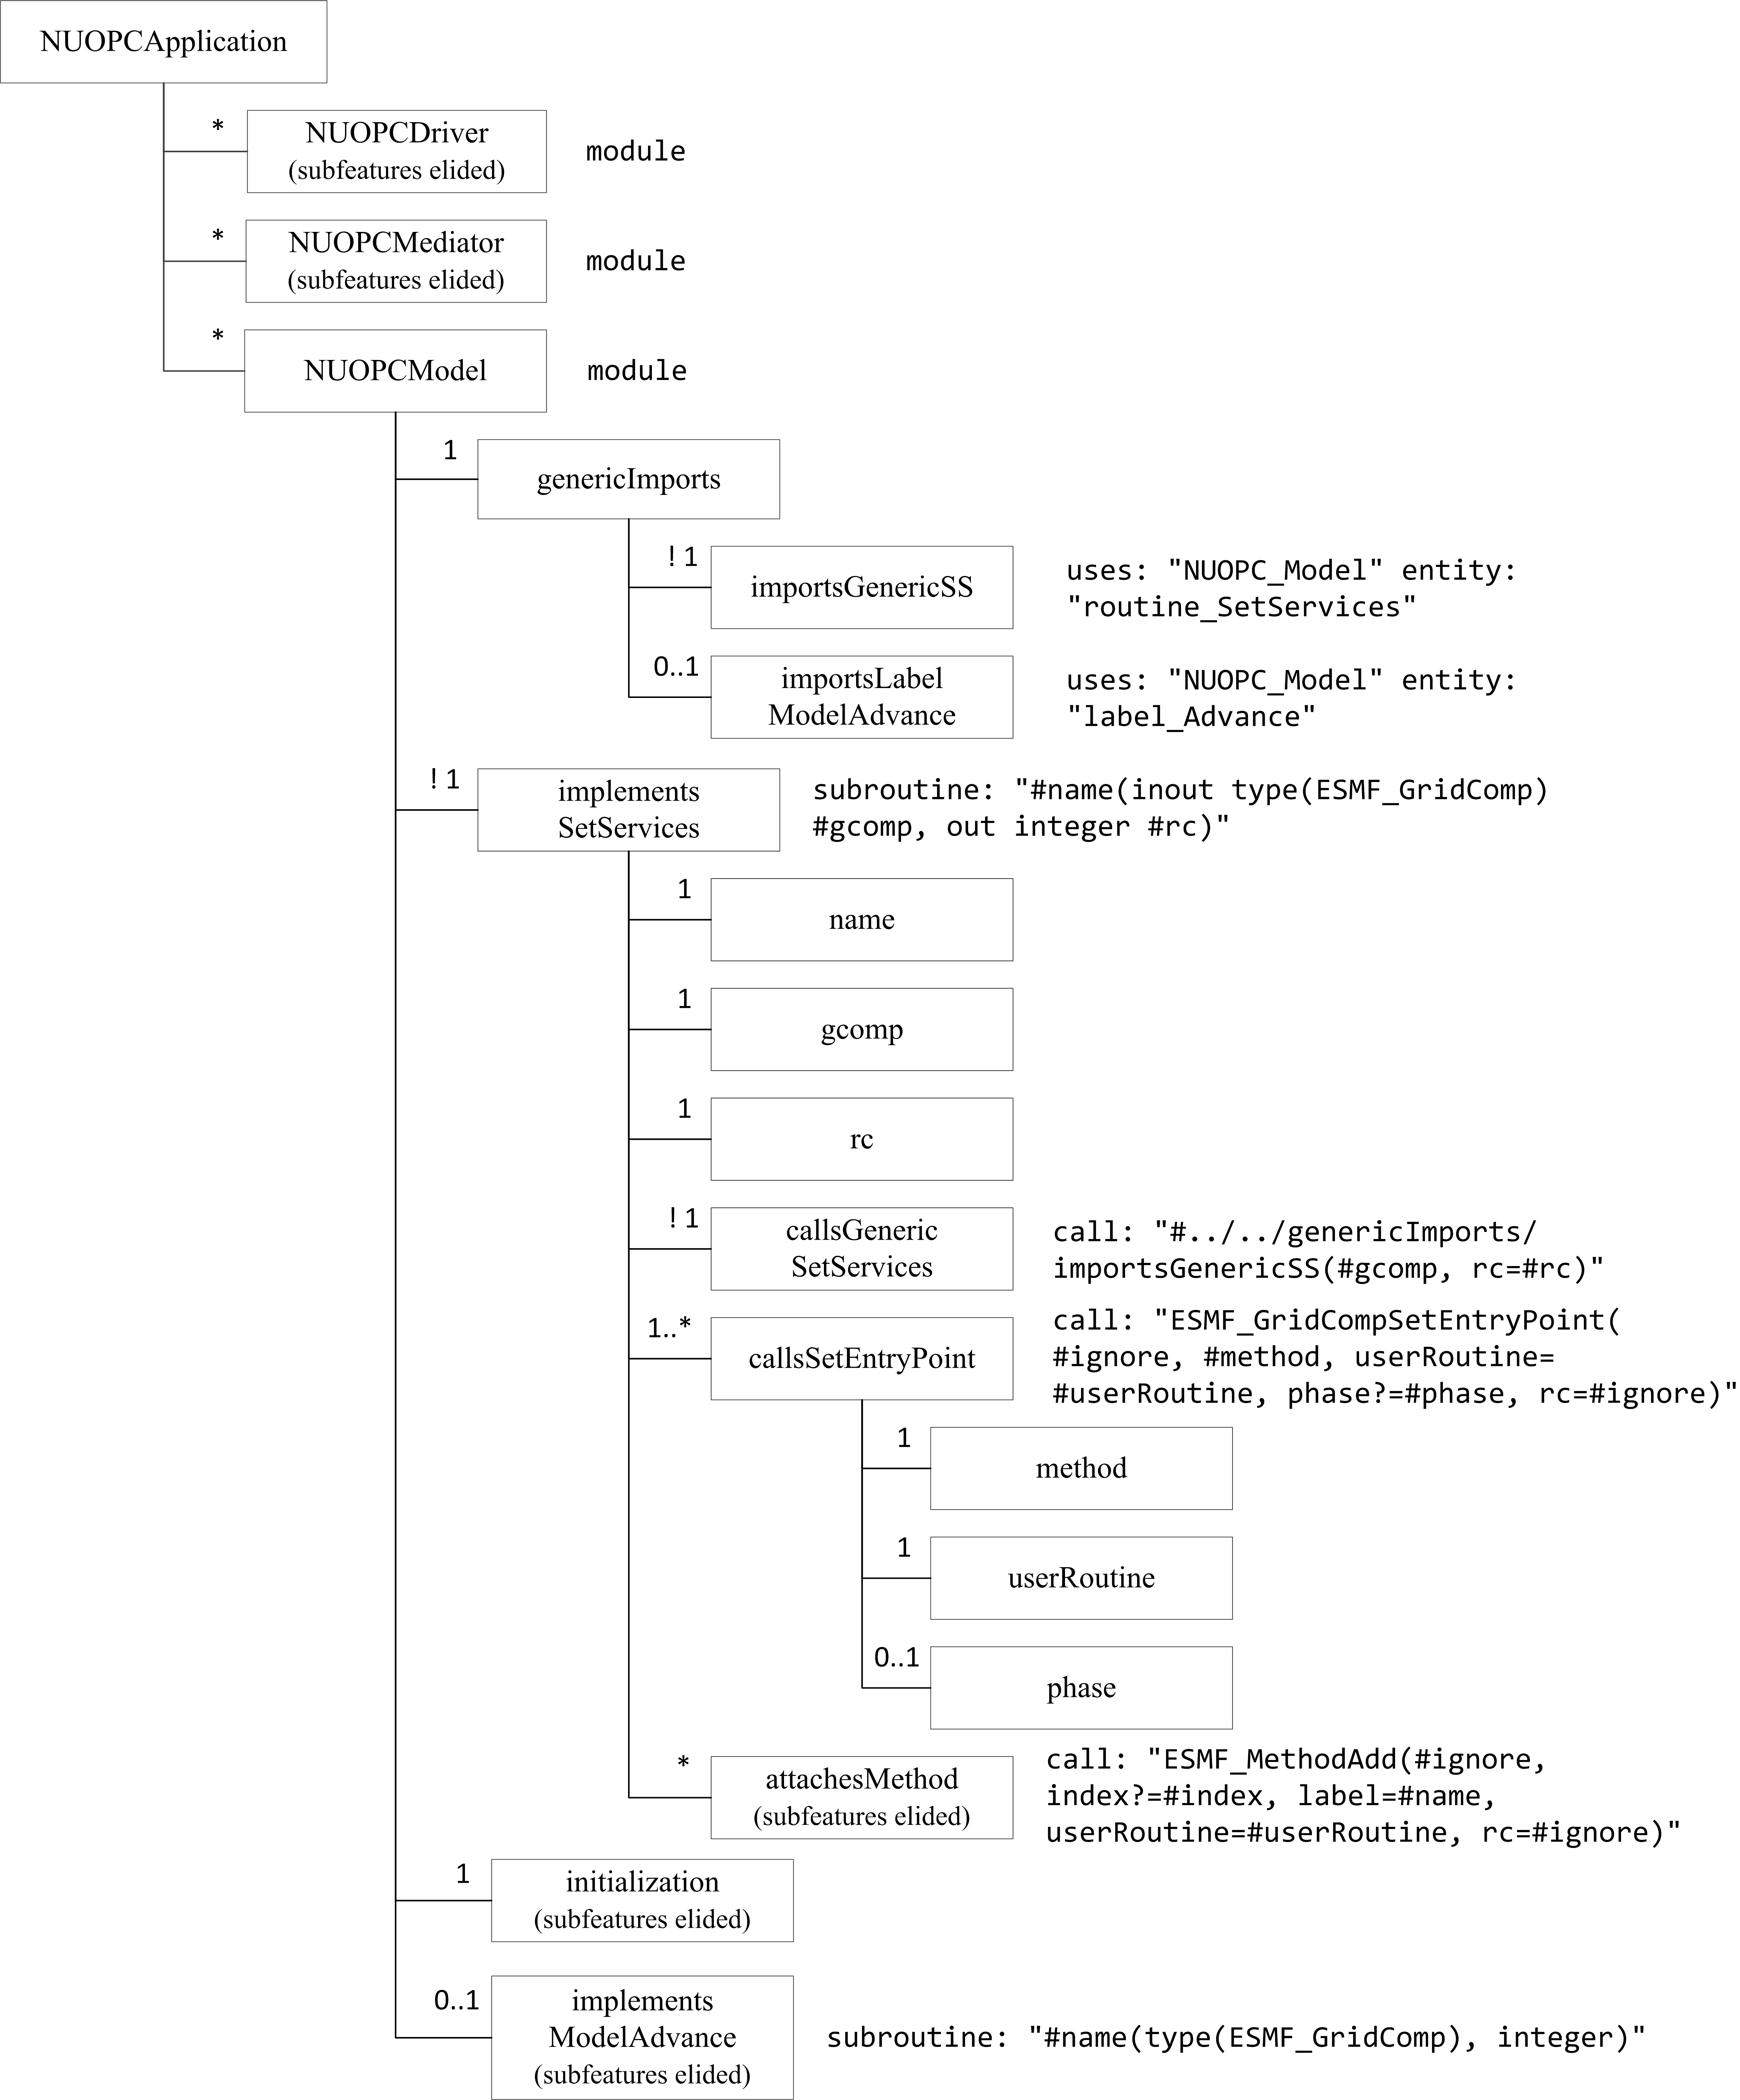
\includegraphics[width=\textwidth]{figs/nuopcfm.png}
	\caption{A partial feature model representation of the NUOPC FSML}
	\label{fig:nuopcfm}
\end{figure}

%\begin{figure}
	%\centering
	 %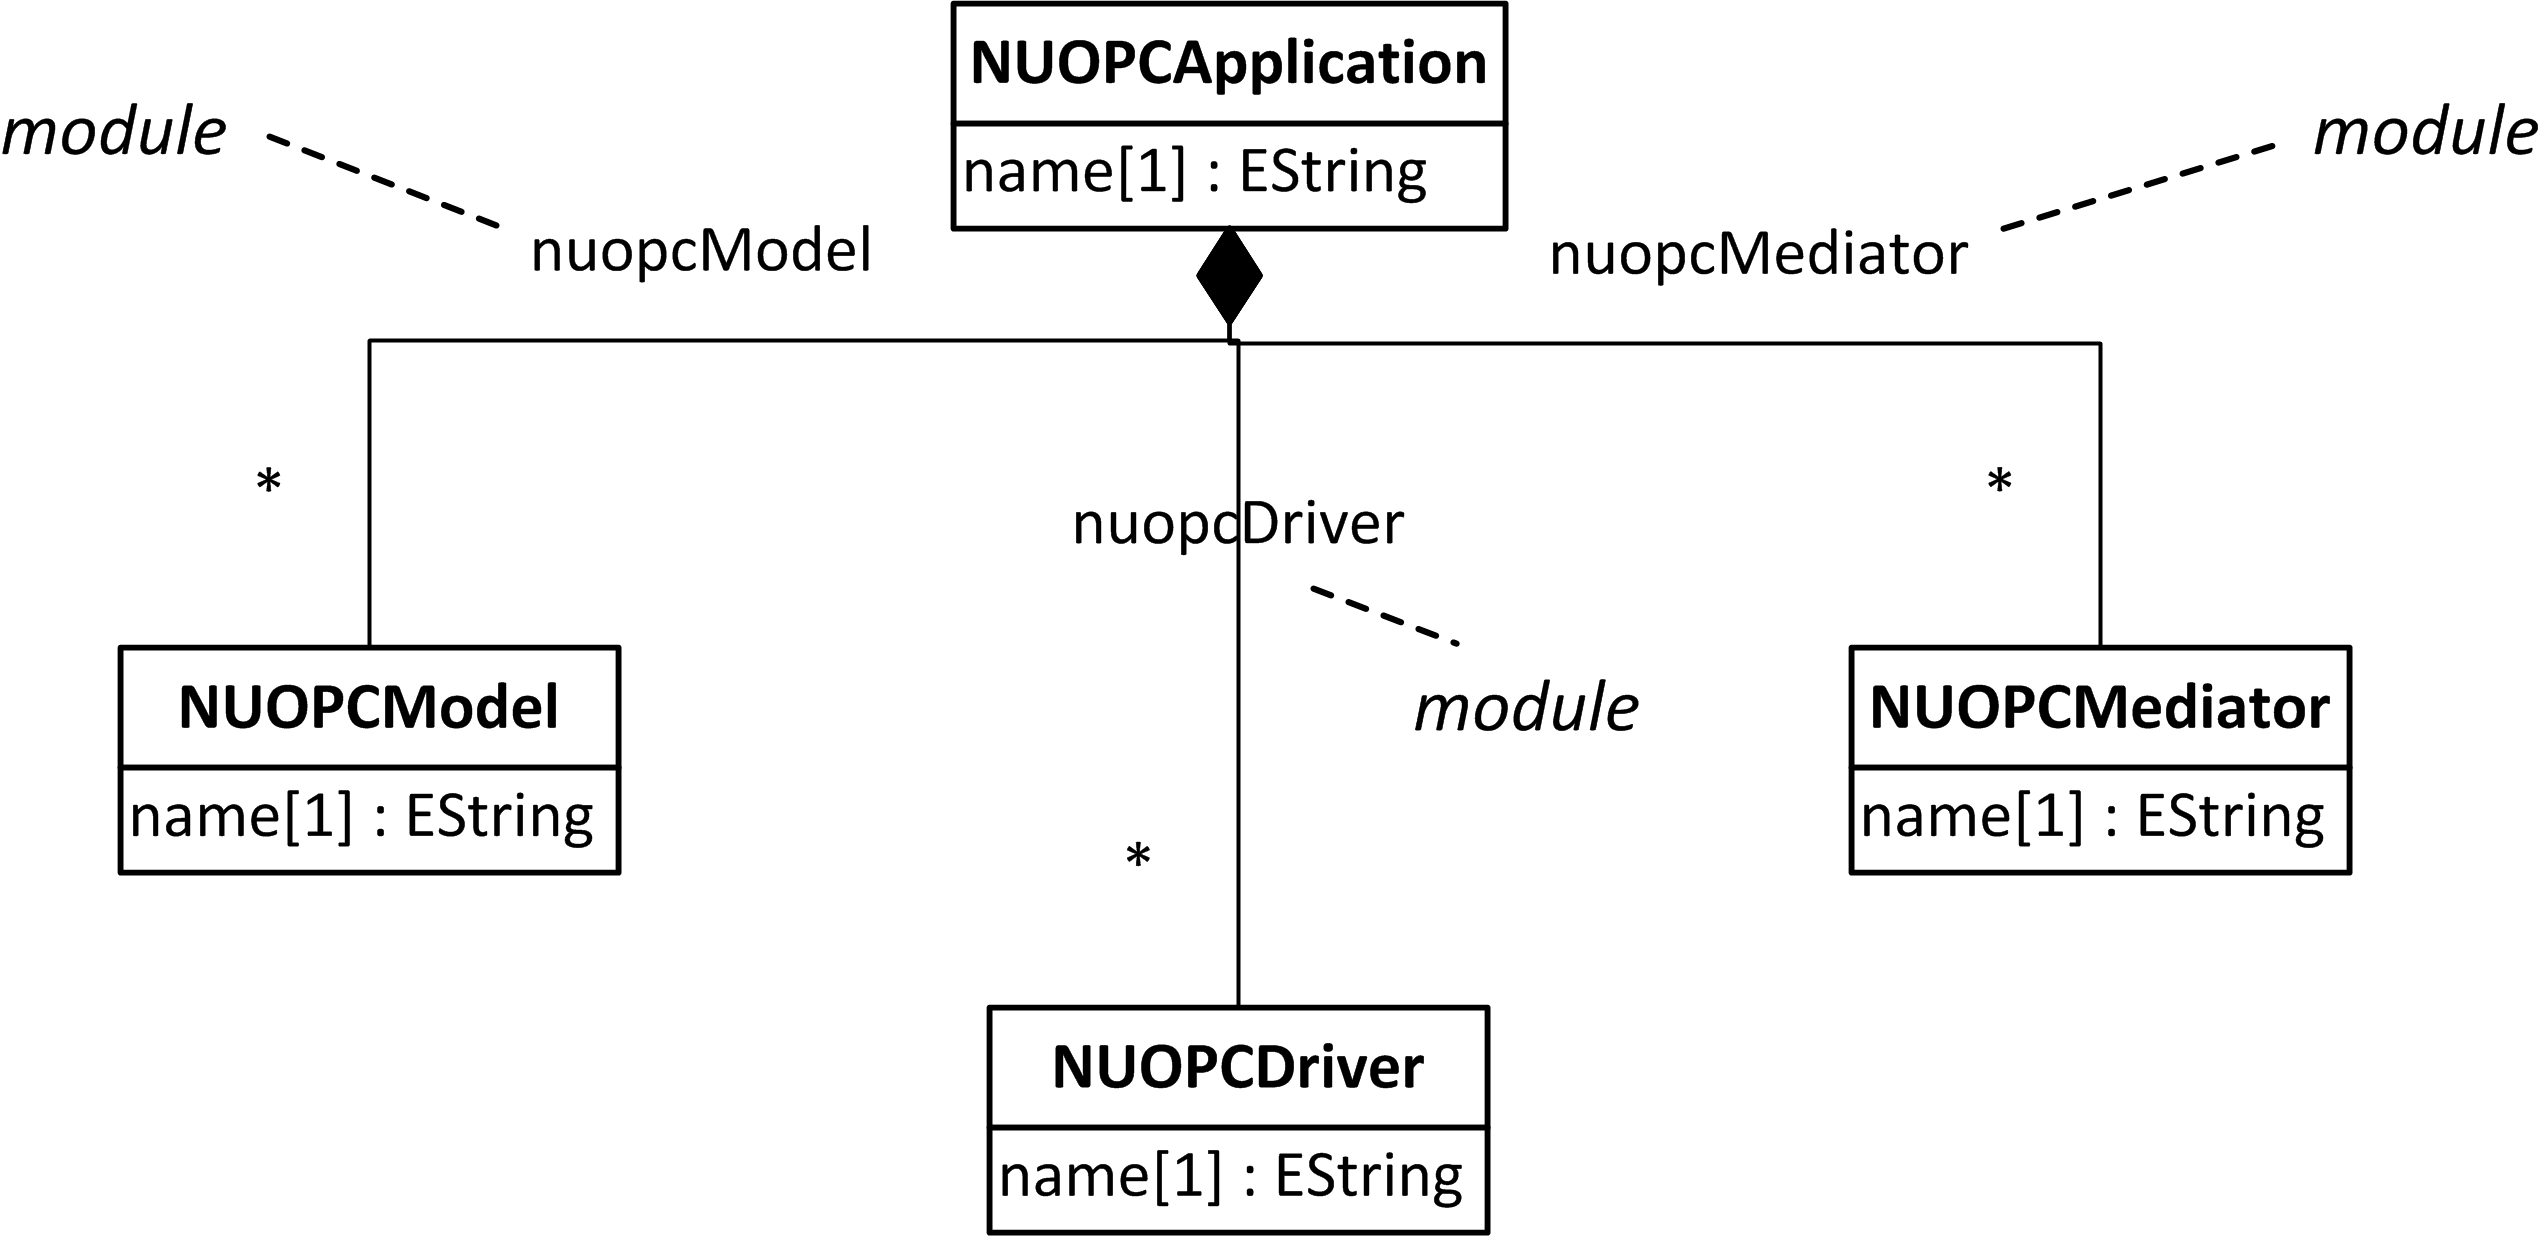
\includegraphics[width=.7\textwidth]{figs/nuopcapp.png}
	%\caption{Top-level classes in the NUOPC Framework Specific Modeling Language (FSML). \texttt{NUOPCApplication} is the top-level class with three containment references: \texttt{NUOPCModel}, \texttt{NUOPCDriver}, and \texttt{NUOPCMediator}. (Some references are not shown.) Mappings from framework-provided concepts to code artifacts are shown in \mapping{italics}.}
	%\label{fig:nuopcapp}
%\end{figure}

This section describes a subset of the abstract syntax of the NUOPC FSML. Figure~\ref{fig:nuopcfm} shows some of the framework-provided concepts in the NUOPC FSML represented as features in a feature model. The top-level concept node is \texttt{NUOPCApplication}. Its child features, \texttt{NUOPCModel}, \texttt{NUOPCDriver}, and \texttt{NUOPCMediator}, are the primary architectural components defined by NUOPC that require specialization by the developer. Subfeatures of \texttt{NUOPCModel} include \texttt{genericImports}, a container feature for required and optional module imports, \texttt{implementsSetServices}, which represents a framework-called subroutine that the developer implements, \texttt{initialization}, whose (elided) subfeatures represent the initialization subroutines that the developer implements, and \texttt{implementsModelAdvance}, which represents the developer-provided subroutine that advances the model forward in time.

\emph{Mapping definitions} define the correspondence between features in the FSML and structural and behavioral code patterns. Cupid defines	 a set of mapping types for Fortran 90, the primary language binding supported by ESMF and NUOPC. Currently, only structural mappings types are supported, and they have been defined on an as-needed basis. Mappings are indicated in the figure next to each feature. \texttt{NUOPCModel}, \texttt{NUOPCDriver}, and \texttt{NUOPCMediator} each have a mapping definition of \texttt{module}. The top-level concept, \texttt{NUOPCApplication}, does not indicate a mapping. It will be implicitly mapped to an entire codebase. (Think of this as the root directory of a source tree.) Table~\ref{tab:mappings} lists the current set of supported mapping types.

The mapping definition for the feature \texttt{implementsSetServices} is \texttt{subroutine: "\#name(inout type(ESMF\_GridComp) \#gcomp, out integer \#rc)"}. A subroutine signature includes the subroutine name, and optionally the intents (in/out/inout), types, and names of its formal parameters. Only subroutines with a matching name and matching argument intents and types are matched. In general, mapping definitions may include meta-variables that refer to features. The subroutine signature above contains three meta-variables, \texttt{\#name}, \texttt{\#gcomp}, and \texttt{\#rc}. The \texttt{\#name} meta-variable implicitly maps the subfeature \texttt{name} to the name of the mapped subroutine.

%When the mapping is executed in the reverse engineering direction, the attributes \texttt{name}, \texttt{gcomp}, and \texttt{rc} are populated by the mapped subroutine name, its first formal parameter name, and its second formal parameter name, respectively.

In the figure, some features are marked with a \texttt{!} indicating that they are \emph{essential} features. A feature is only instantiated if all of its essential child features can be successfully mapped. For example, in Figure~\ref{fig:nuopcfm}, the features \texttt{importsGenericSS} and \texttt{callsGenericSetServices} are essential. If their mappings fail, then the higher-level feature \texttt{NUOPCModel} will not be be instantiated.

{
\footnotesize
\begin{table}
\caption{Mappings types for Fortran 90}
\label{tab:mappings}
\begin{center}
    \begin{tabular}{| l | p{8cm} |}
		\hline
    \textbf{Structural Pattern Expression} & \textbf{Structural Elements Matched} \\ \hline
		\texttt{module} & matches a Fortran module \\ \hline
		\texttt{m moduleName} & matches the name of module \texttt{m} \\ \hline
		\texttt{m usesModule: mn} & matches use statements in module \texttt{m} with imported module name \texttt{mn} \\ \hline
		\texttt{u usesEntity: en} & matches import of entity named \texttt{en} within use statement \texttt{u} \\ \hline
		\texttt{m uses: mn entity: en} & matches use statements in module \texttt{m} with imported module name \texttt{mn} and imported entity name \texttt{en} \\ \hline
		\texttt{m subroutine} & matches subroutines defined within module \texttt{m} \\ \hline
		\texttt{m subroutine: ss} & matches subroutines defined within module \texttt{m} with signature \texttt{ss} \\ \hline
		\texttt{s subroutineName} & matches the name of subroutine \texttt{s} \\ \hline
		\texttt{s formalParam: i} & matches the \texttt{i}th formal parameter of subroutine \texttt{s} \\ \hline
		\texttt{s call} & matches calls with the implementation of subroutine \texttt{s} \\ \hline
		\texttt{s call: cs} & matches calls with the implementation of subroutine \texttt{s} with call signature \texttt{cs}\\ \hline
		\texttt{c argByIndex: i} & matches the \texttt{i}th actual parameter of call \texttt{c} \\ \hline
		\texttt{c argByKeyword: k} & matches the actual parameter with keyword \texttt{k} of call \texttt{c} \\ \hline
    \end{tabular}
\end{center}
\end{table}
}


\section{FSML Implementation}

In Cupid, a FSML is implemented as an Ecore model to take advantage of the Eclipse Modeling Framework (EMF) suite of tools. Ecore is an object-oriented meta-model and it includes a graphical Eclipse-based editor for creating class models and generating Java code. While classes represent framework-provided concepts, annotations on classes and their properties are used to specify mapping definitions. Figure~\ref{fig:nuopcmodel} shows a UML class diagram for part of the NUOPC FSML rooted at the feature \texttt{NUOPCModel}. Features are represented as classes or attributes and subfeatures are represented as containment references. Figure~\ref{fig:setservices_mappings} shows an instantiation of classes (a FSM) and mappings to source code.

\begin{figure}
	\centering
	 \makebox[\textwidth][c]{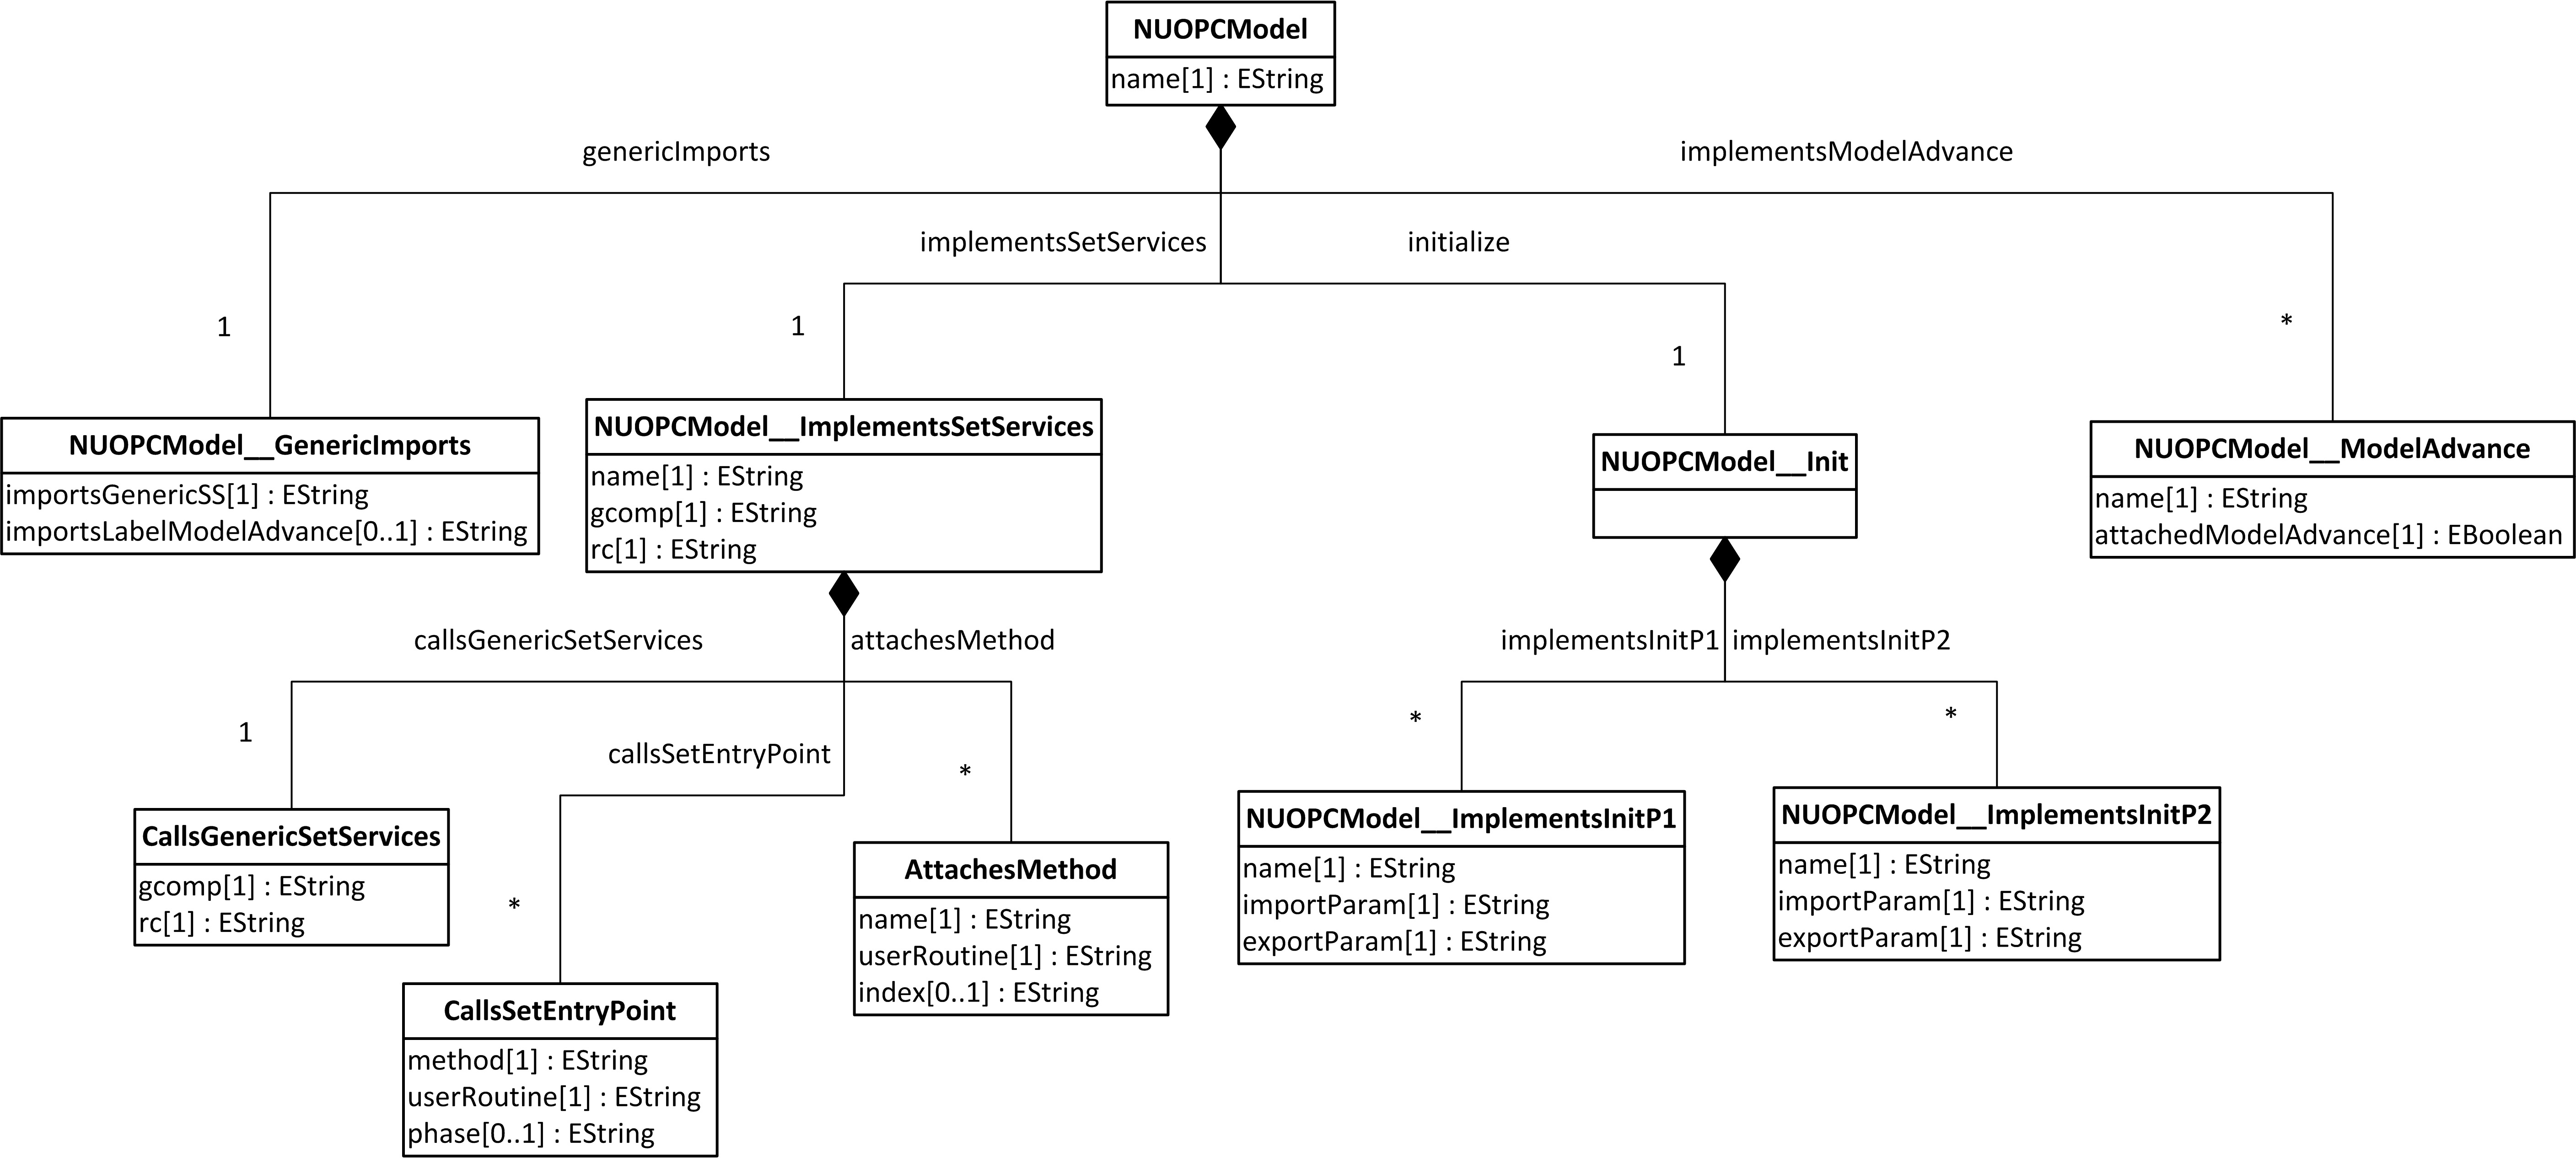
\includegraphics[width=1.1\textwidth]{figs/nuopcmodel.png}}
	 \caption{Partial NUOPC FSML class diagram rooted at \texttt{NUOPCModel}.}
	\label{fig:nuopcmodel}
\end{figure}

\begin{figure}
	\centering
	 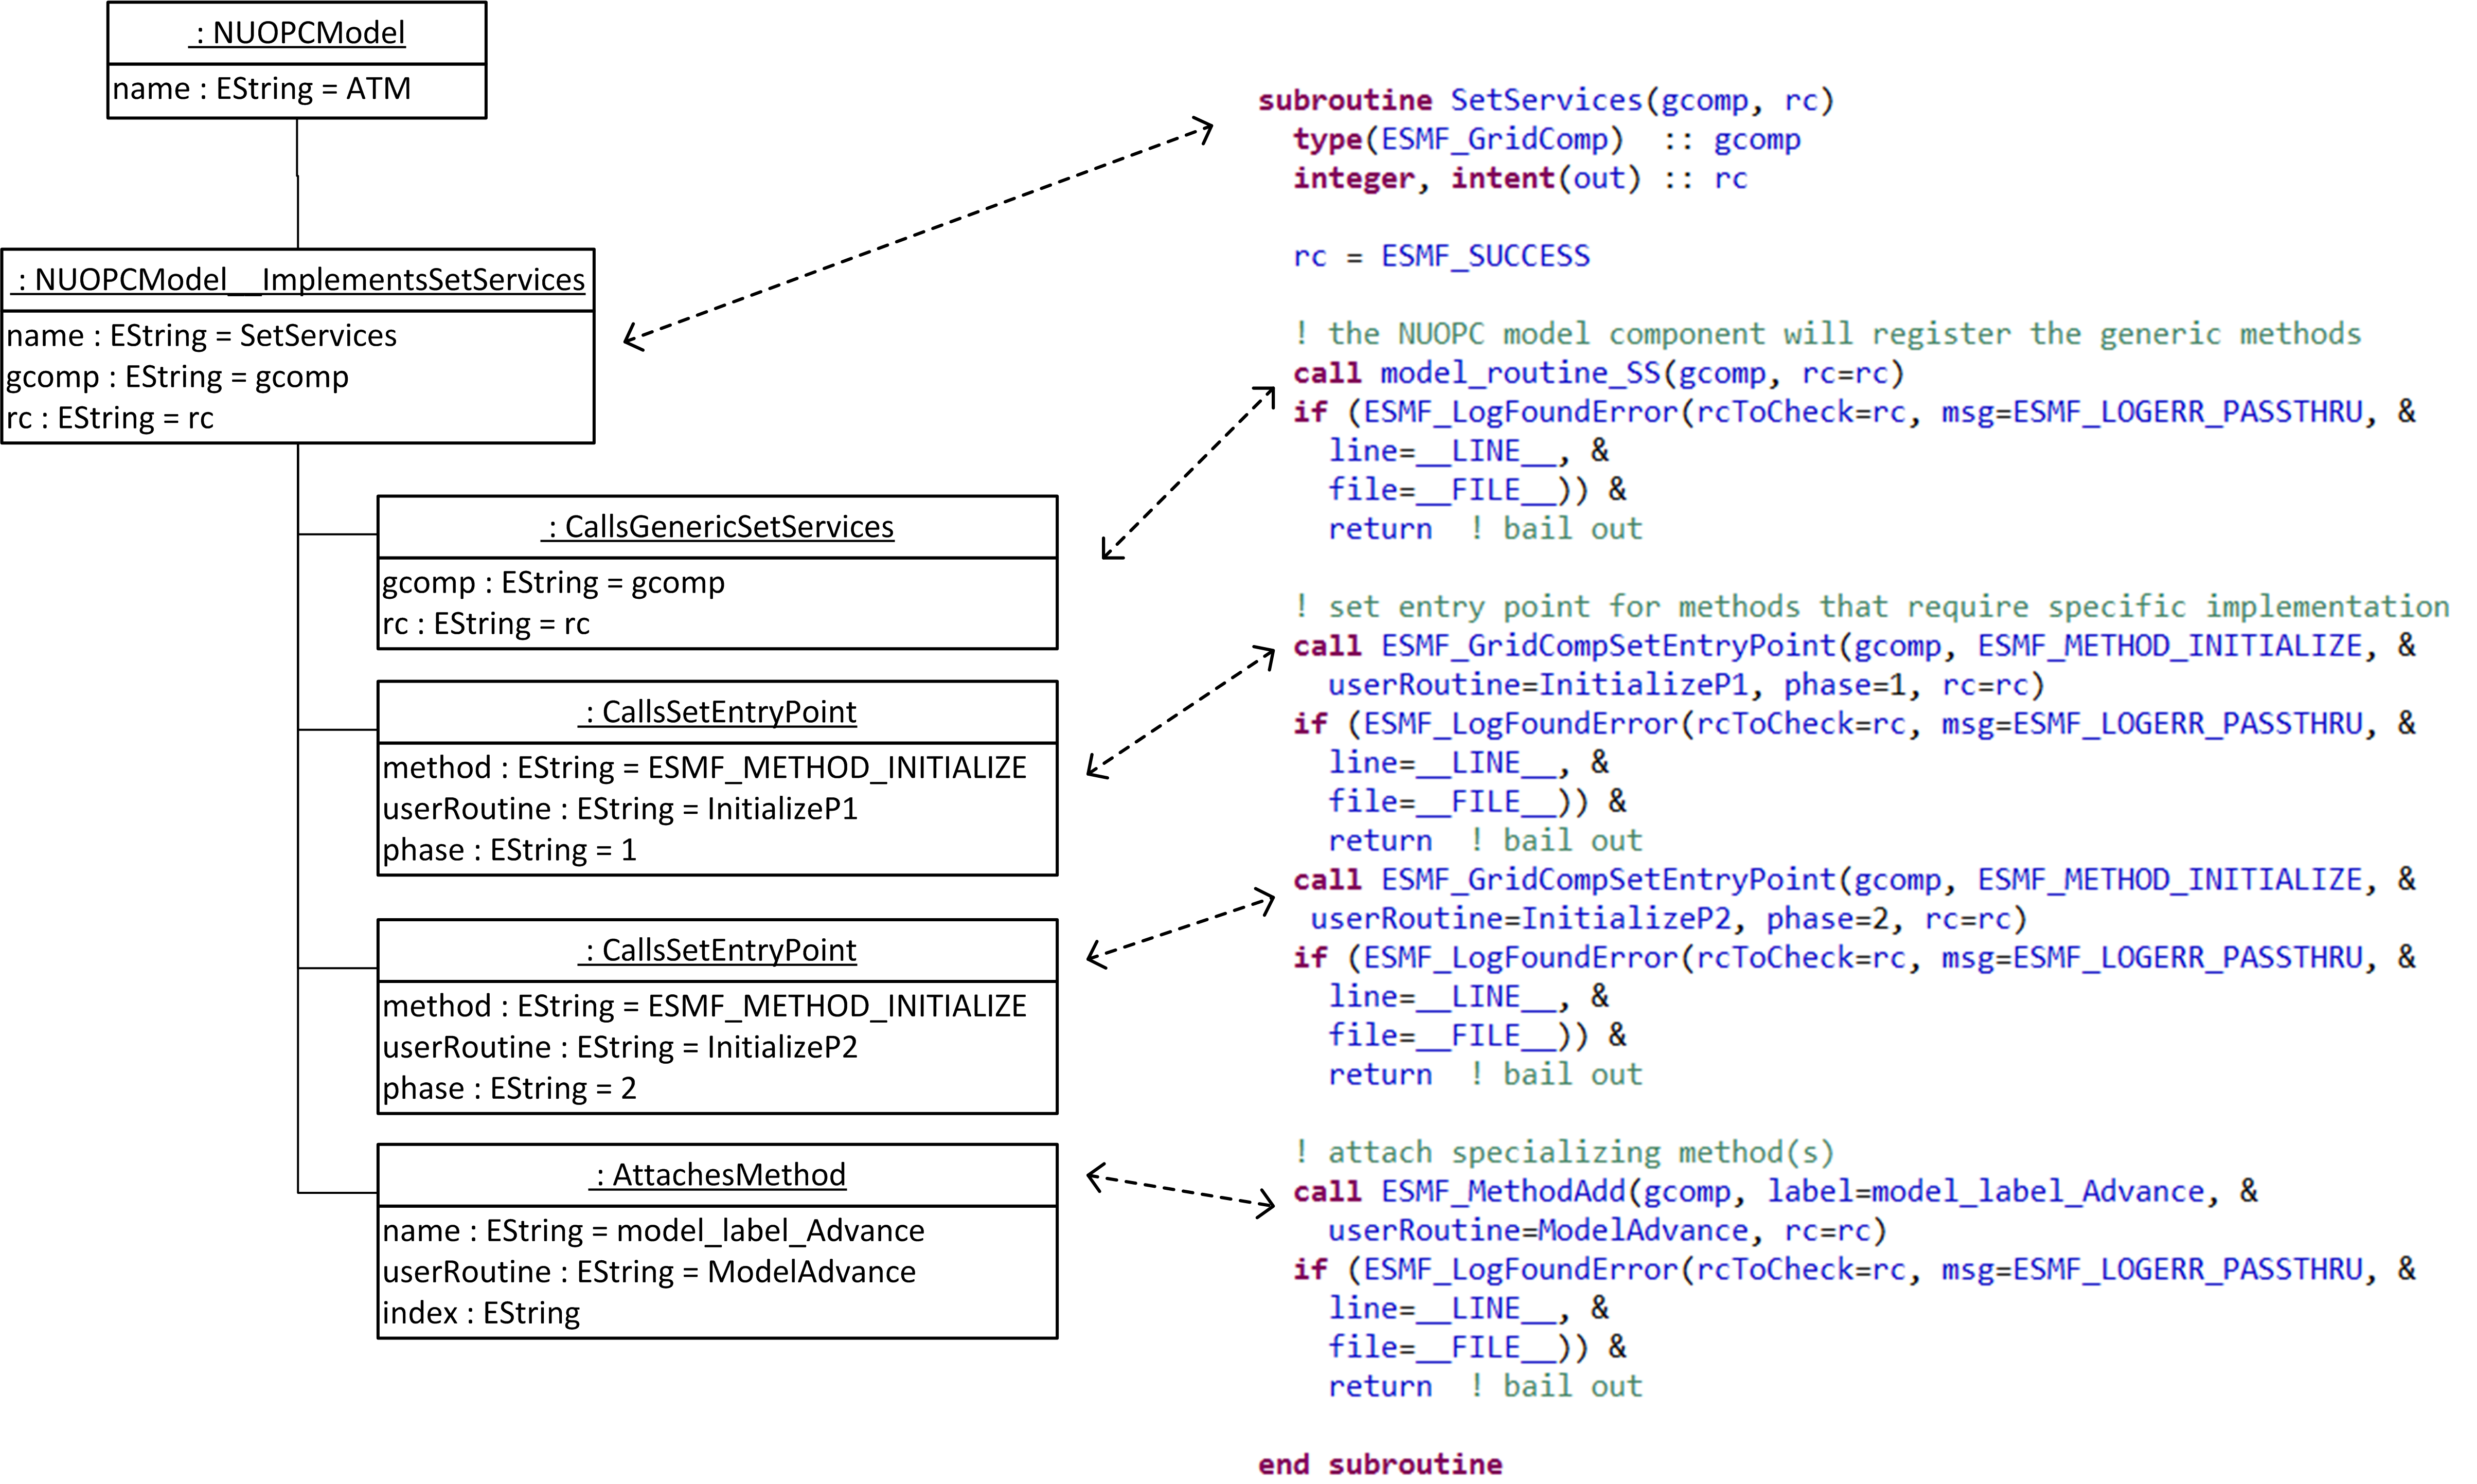
\includegraphics[width=1.1\textwidth]{figs/setservices_mappings.png}
	\caption{The object diagram on the left shows an instantiation of part of the NUOPC FSML corresponding to a \texttt{Model SetServices} subroutine. The dashed lines show mappings from FSM objects to source code.}
	\label{fig:setservices_mappings}
\end{figure}






\bibliographystyle{plain}
\bibliography{bib}

\end{document}